\documentclass[11pt]{article}
\usepackage[utf8]{inputenc}
\usepackage[spanish]{babel}
\usepackage{amsmath}
\usepackage{natbib}
\usepackage{float}
\usepackage{graphicx}
\usepackage[hidelinks]{hyperref}
\usepackage{listings}
\usepackage{caption}
\usepackage{url}
\graphicspath{ {img/} }
\title{Planificador con algoritmo genético}
\author{Borja Bares Fernández}
\date{}

\renewcommand{\lstlistingname}{Código}
\captionsetup[lstlisting]{position=bottom, belowskip=\baselineskip}

\begin{document}
	
	\maketitle
	
	\section{Descripción del problema}
	
	En un taller de postventa de vehículos se realizan muchas operaciones y la planificación de estas es una tarea compleja.
	
	Simulando un taller con operaciones ya planificadas con antelación se deben planificar operaciones para un nuevo vehículo en un solo día partiendo de las siguientes suposiciones:

	\begin{itemize}
		\item El tiempo del taller se divide en intervalos de 30 minutos.
		\item El taller puede planificar operaciones de 00:00 a 23:59.
		\item El taller tiene varios empleados.
		\item Todos los empleados pueden realizar todas las operaciones.
	\end{itemize}
	
	Además las tareas a planificar deben cumplir ciertas restricciones:
	
	\begin{itemize}
		\item Un empleado no puede realizar dos o más operaciones a la vez.
		\item Dos operaciones a planificar no pueden realizarse a la misma hora por distintos empleados ni solaparse.
		\item Si es posible, un mismo empleado realizará varias operaciones seguidas sobre el vehículo para minimizar tiempos perdidos entre cambios de vehículos, a pesar de que estos tiempos se ignoren en este problema.
	\end{itemize}
	
	Con todo esto el planificador intentará asignar operaciones a empleados intentando minimizar el tiempo que el coche está en el taller. 
	
	Ya que suponemos que el coche se ha recepcionado en otro día anterior al que se intentan planificar las operaciones, el planificador intentará que las operaciones acaben lo más pronto posible.
	
	\section{Representación del cromosoma}
	
	Para representar el cromosoma se ha creado un array con tantas posiciones como huecos hay para planificar en un día. Al planificar operaciones de 30 en 30 minutos hay 48 posiciones por empleado.
	
	\begin{figure}[h]
		\centering
		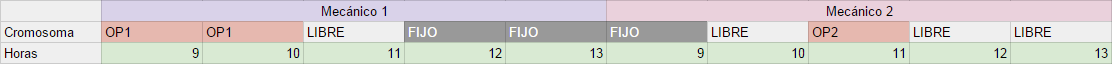
\includegraphics[width= 12.5cm]{cromosoma.png}
		\caption{Representación simplificada de un cromosoma.}
	\end{figure}
	
	
	Sobre esta representación es muy sencillo realizar operaciones ya que se puede obtener muy fácilmente tanto la posición dentro de un empleado como el empleado que tiene que realizar la operación.
	
	\section{Mutaciones}
	Las mutaciones que se realizan sobre el cromosoma son siempre sobre una operación a planificar seleccionada de forma aleatoria. Los huecos reservados\footnote{Operaciones que ya estaban planificadas de antes.} no se desplazan.
	
	Sobre la operación a modificar se pueden realizar dos tipos de mutaciones. El tipo de mutación que se realiza se escoge al azar. La probabilidad de escoger una u otra se va modificando en el tiempo para intentar favorecer que las operaciones se asignen al mismo empleado.
	
	Los tipos de mutaciones son las siguientes:
	
	\subsection{Cambio de slot}
	
	Entendemos como slot un hueco de 30 minutos de un empleado.
	
	Este desplazamiento se hace de forma aleatoria impidiendo ya en la mutación los siguientes casos:
	
	\begin{itemize}
		\item Que la operación se planifique sobre un hueco reservado.
		\item Que las operaciones colisionen unas con otras.
		\item Que la operación termine fuera del cromosoma.
	\end{itemize}
	
	\subsection{Cambio de empleado}
	
	A medida que se avanza en la planificación se favorece este tipo de mutación.
	
	En las pruebas realizadas, en ocasiones el algoritmo acababa con soluciones bastante buenas del siguiente estilo:
	
	\begin{figure}[h]
		\centering
		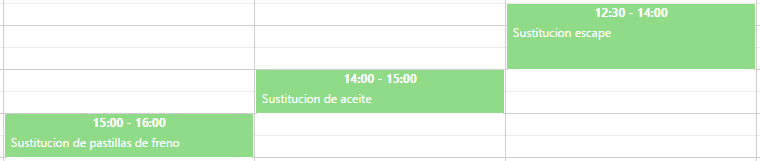
\includegraphics[width= 12.5cm]{ejemplo-unidades.png}
		\caption{Ejemplo de planificación no deseada.}
		\label{ejemplo-unidades}
	\end{figure}
	
	Este tipo de planificación no era la deseada, ya que ambos empleados tienen tiempo disponible y se deseaba que en caso de poder permitírselo todas las operaciones las realizase un empleado.
	
	Al mover las operaciones a slots aleatorios el algoritmo solía acabar sin encontrar una solución mejor, por eso se creó este tipo de mutación en la que una operación se cambia de empleado sin moverla en el tiempo.
	
	En las pruebas realizadas los resultados son más satisfactorios.
	
	\section{Cruce}
	
	Inicialmente se contempló realizar operaciones de cruce, aunque posteriormente se desechó esta idea ya que podía dar lugar con mucha probabilidad a cromosomas no válidos.
	
	Los cromosomas no válidos que se contemplaron podría tener operaciones duplicadas u operaciones cortadas por la mitad haciendo que todos sus descendientes no fuesen ya válidos.
	
	\section{Evaluación del cromosoma}
	
	Para la evaluación del cromosoma se tienen en cuenta ciertas características para penalizarlas.
	
	Cada característica tiene un factor que determina cuánto penaliza su aparición en la calidad global del cromosoma.
	
	Inicialmente se había pensado en añadir una hora para iniciar la planificación y penalizar que hubiese operaciones antes de esa hora, al final se desechó esa idea ya que bastaría con no incluir esas horas en el cromosoma.
	
	\subsection{Hora de final de la última operación} 
	
	El objetivo del planificador es acabar cuanto antes con el vehículo de manera que se obtiene el último slot de la última operación y se utiliza como penalización.
	
	\subsection{Cantidad de slots solapados}
	
	\begin{figure}[h]
		\centering
		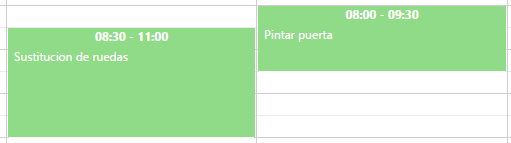
\includegraphics[width= 9cm]{ejemplo-solapamiento.png}
		\caption{Dos operaciones con dos huecos solapados.}
	\end{figure}
	
	Sobre un vehículo no se pueden realizar dos operaciones a la vez. A diferencia del resto de características esta era excluyente, ya que el resto hacen que una solución sea mejor o peor, esta hace que una solución no sea válida.
	
	Este caso se ha penalizado de forma muy agresiva y aún así hay situaciones concretas en las que sigue apareciendo.
	
	\subsection{Huecos entre operaciones}
	
	\begin{figure}[h]
		\centering
		
\includegraphics[width= 9cm]{ejemplo-hueco.png}
		\caption{Huecos entre operaciones.}
		\label{ejemplo-hueco}
	\end{figure}
	
	Se ha penalizado los huecos que hay entre operaciones, tanto si están en el mismo empleado como entre empleados. 
	
	Esta penalización va decreciendo a medida que el hueco está más alejado del inicio del día. Esto es así ya que como se puede ver en el ejemplo de la figura \ref{ejemplo-hueco} el algoritmo se quedaba atascado. Al mover una operación de cada vez, si se movía la operación de \textit{Sustitución de aceite}, seguía habiendo el mismo número de huecos. La última operación seguía estando en el mismo punto de manera que ambos cromosomas tenían la misma calidad, desechándose el nuevo que podía dar a que la última posición se planificase de 18:30 a 19:30.
	
	\subsection{Huecos desde el inicio del día hasta la primera operación}
	
	Se escogió penalizar el inicio de las operaciones en el coche ya que, penalizando solamente los huecos entre operaciones, se daban casos en los que, aún habiendo huecos libres, las operaciones no empezaban a las 00:00 si no que se retrasaban una o dos horas.
	
	\subsection{Cambios de operario}
	
	Como ya se explicó en mutaciones, la planificación mostrada en la figura \ref{ejemplo-unidades} no es la deseada. 
	
	Dado que los algoritmos genéticos tienen un componente aleatorio, las operaciones siempre aparecían \textit{desperdigadas} entre los operarios, esto no es deseable ya que tanto si los mecánicos se tienen que cambiar de box o se tiene que desplazar el vehículo se pierde mucho tiempo.
	
	Para evitar esto se penalizan los cambios de operarios.
	
	\section{Algoritmo}
	
	El algoritmo genera mutaciones a partir de un cromosoma inicial creado de forma aleatoria. Esto es así hasta que ha pasado un minuto o hasta que se pasan cierto número de iteraciones sin encontrar un cromosoma mejor que el actual. 
	
	El número de iteraciones para que el algoritmo finalice se ha escogido haciendo ejecuciones de prueba con distintos escenarios y buscando un valor lo suficientemente cercano al mayor número de iteraciones necesarias para encontrar una solución mejor a la actual.
	
	Con cierta probabilidad se seleccionan soluciones peores a la actual. Esta solución peor no puede ser peor que un límite marcado a partir del primer cromosoma, este límite va decreciendo a medida que se van generando mutaciones. Esta idea está sacada del algoritmo \textit{great deluge}.
	
	\section{Como usar el algortimo}
	
	Para ejecutar el programa es necesario tener instalado \textit{Java 8} y \textit{Maven}\footnote{\url{http://maven.apache.org}}.
	
	Una vez comprobado que tenemos todo instalado y funcionando desde un \textit{terminal} iremos a la carpeta que contiene el archivo \textit{pom.xml} y la carpeta \textit{src} y escribiremos:
	
	\begin{lstlisting}[language=bash]
	$mvn jetty:run
	\end{lstlisting}
	\captionof{lstlisting}{Ejecución del algoritmo con \textit{Maven}.}
	
	
	En cuanto nos aparezca el siguiente mensaje podremos conectarnos desde un navegador web a la dirección \url{http://localhost:8080}.
	
	\begin{lstlisting}[language=bash]
	[INFO] Started Jetty Server
	\end{lstlisting}
	\captionof{lstlisting}{El servidor está iniciado.}
	
	Desde esta dirección debemos por lo menos añadir un nuevo hueco ocupado haciendo doble click, esto es importante, ya que el planificador toma el día en el que está ese hueco como el día en el que tiene que planificar. Por lo tanto también es importante no poner huecos ocupados en otros día.
	
	Los \textit{huecos ocupados} que aparecen en el planificador se pueden desplazar y modificar en duración.
	
	Para iniciar el proceso de planificación se debe pulsar el botón de \textit{Mostrar formulario de cita} situado arriba a la derecha de la pantalla, posteriormente seleccionar operaciones y darle al botón \textit{Planificar}.
	
	Durante el proceso de planificación, las operaciones a planificar aparecerán en amarillo y se moverán, es importante no desplazar ni modificar la duración de esas operaciones ya que el planificador podría no funcionar de forma correcta.
	
	En cuanto se acabe la planificación las operaciones pasarán a ser de color verde.
	
	Una vez finalizado el proceso de planificación se puede repetir de la misma forma, o si se desea, se puede recargar de nuevo la página, lo que hará que las operaciones planificadas desaparezcan. 
	
	En caso de que al recargar la página aparezcan operaciones no planificadas una vez haya acabado la planificación, se recomienda reiniciar el servidor.
	
	Se adjunta además para la ejecución de la práctica un archivo \textit{ROOT.war} que puede ser ejecutado en cualquier servidor de \textit{servlets}, como por ejemplo \textit{Tomcat}.
	
	\section{Conclusiones}
	
	Que el algoritmo funcione es realmente sencillo, ya que casi sin esfuerzo se obtienen soluciones al problema. La dificultad viene cuando se empiezan a afinar estas soluciones.
	
	En mi caso, he encontrado ocasiones en las que el algoritmo no hacía lo que yo esperaba y no lograba determinar qué estaba pasando. Esto me llevó a añadir nuevos tipos de mutaciones, modificaciones en el bucle que las genera o elementos para penalizar la calidad del cromosoma para posteriormente darme cuenta que era otra cosa.
	
	También he dedicado mucho tiempo a buscar valores correctos para los factores de las penalizaciones, iteraciones de los bucles y similares, ya que hay que llegar a un compromiso entre ellos. El problema viene con la amplia cantidad de posibles combinaciones de operaciones, ya que esto dificulta saber si se están penalizando casos muy concretos e ignorando otros.
	
	Me hubiese gustado mejorar los factores anteriormente seleccionados para que tengan en cuenta el periodo que se planifica, el tamaño de los slots, el número de operaciones a planificar y el número de operarios. Me da la impresión de que todos los valores que he asignado para que el algoritmo funcione bien se pueden expresar teniendo en cuenta esos valores, haciendo que este acepte un mayor número de configuraciones.
	
	También me gustaría indicar que la interfaz del planificador, así como el uso de esta, tiene unos cuantos bugs o requisitos poco deseables\footnote{No poder tener operaciones en varios días, no poder borrar operaciones \ldots}. Esto es así ya que he procurado no dedicar más tiempo a la parte de interfaz que al algoritmo genético.
	
\end{document}